\documentclass[xcolor={usenames,dvipsnames,svgnames}, compress]{beamer}

% \usepackage[utf8]{inputenc}
\usepackage{booktabs}
\usepackage{dcolumn}
\usepackage{colortbl}
\usepackage{hyperref}

% \usepackage[style=authoryear-comp, backref=true]{biblatex}
\usepackage{ifxetex}
\usepackage{amsmath}
\usepackage{biblatex}
% 
\usepackage[no-math]{fontspec}

\definecolor{jess-fucsia}{RGB}{170, 0, 127}
\definecolor{violent-green}{RGB}{0, 128, 96}
\definecolor{ny-orange}{RGB}{255, 128, 0}

\hypersetup{
  colorlinks=true,       % false: boxed links; true: colored links
  linkcolor=jess-fucsia,          % color of internal links (change box color with linkbordercolor)
  % citecolor=green,        % color of links to bibliography
  %filecolor=magenta,      % color of file links
  urlcolor=jess-fucsia           % color of external links
}

%%% Local Variables:
%%% mode: latex
%%% TeX-master: t
%%% End:



\usetheme{enziteto}

\setbeamertemplate{headline}{}

%%%%%%%%%%%%%%%%%%%%%%%%%%%%%%%%%%%%%%%%%%%%%%%%%%%%%%%%%%%% 
%%%%%%%%%%%%%%%%%%%%%%%%%%%%%%%%%%%%%%%%%%%%%%%%%%%%%%%%%%%% 
%%%%%%%%%%%%%%%%%%%%%%%%%%%%%%%%%%%%%%%%%%%%%%%%%%%%%%%%%%%% 


\begin{document}

\title{Rule and Knowledge-Based Systems}
\subtitle{A brief introduction}
\author{Antonio Vergari}
% \institute{Lacam$@$DIB$@$Uniba}
\institute{Università degli Studi di Bari}
\department{Dipartimento di Informatica}
\laboratory{LACAM}
\group{Machine Learning}
\institutelogo{
\includegraphics[width=25pt]{Figures/unibaba}}
\lablogo{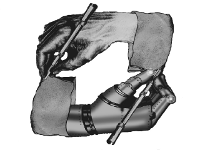
\includegraphics[width=35pt]{Figures/lacam}}

\footnotesize \let\small\footnotesize





{
  \setbeamertemplate{headline}{}
  \setbeamertemplate{footline}{}
  \begin{frame}
    \titlepage
  \end{frame}
}


\section{Context \& Background}
{\setbeamertemplate{headline}{}
  \begin{frame}
    \sectionpage
  \end{frame}
}

\begin{frame}
  \frametitle{Rule-Based Systems}
  
  Different kinds of use for rules in the programming world\footnote{http://www.w3.org/2000/10/swap/doc/rule-systems}:
  \begin{description}
  \item[\textbf{derivation}] as in deductive systems and theorem provers
  \item[\textbf{transformation}] as in rewriting systems, grammars
  \item[\textbf{constraint}] declaration as in Business Rules Management Systems (BRMS)
  \item[\textbf{reaction}] as in the \textsf{ECA} paradigm, e.g. db triggers
  \end{description}\bigskip
  
  
  Rule-based programming falls into the \textbf{definitional programming
  approach} (or declarative programming paradigm, like \emph{logical programming} and
  \emph{purely functional programming}). Programmers write rules,
  demanding a rule \textbf{inference engine} to manage, activate,
  process them.\par\bigskip
  
  There are also meta-languages to express and serialize rules: \href{http://wiki.ruleml.org/index.php/RuleML_Home}{\textsf{RuleML}}.
\end{frame}



\begin{frame}
  \frametitle{Rule Engine Architectures}
  \framesubtitle{what you are expected to know}
  \begin{center}
    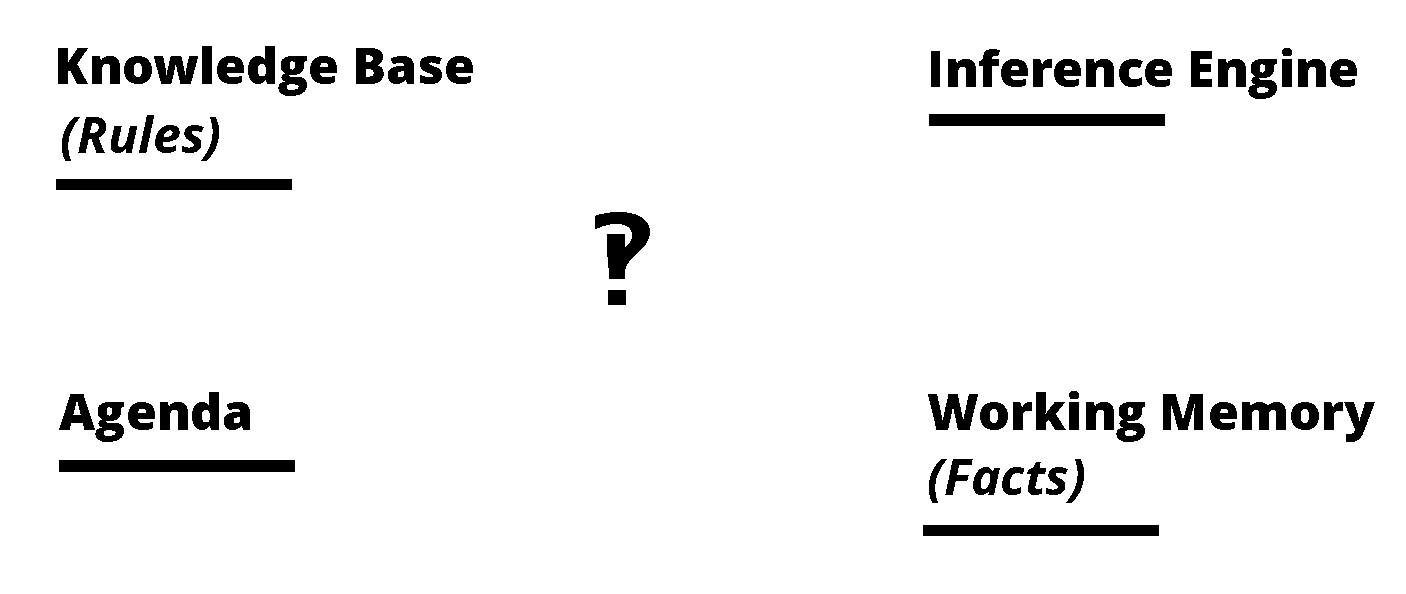
\includegraphics[width=0.8\textwidth]{Figures/es-arch-?}
  \end{center}
\end{frame}

\begin{frame}
  \frametitle{Architectures}
  \framesubtitle{what you are expected to know}
  \begin{center}
    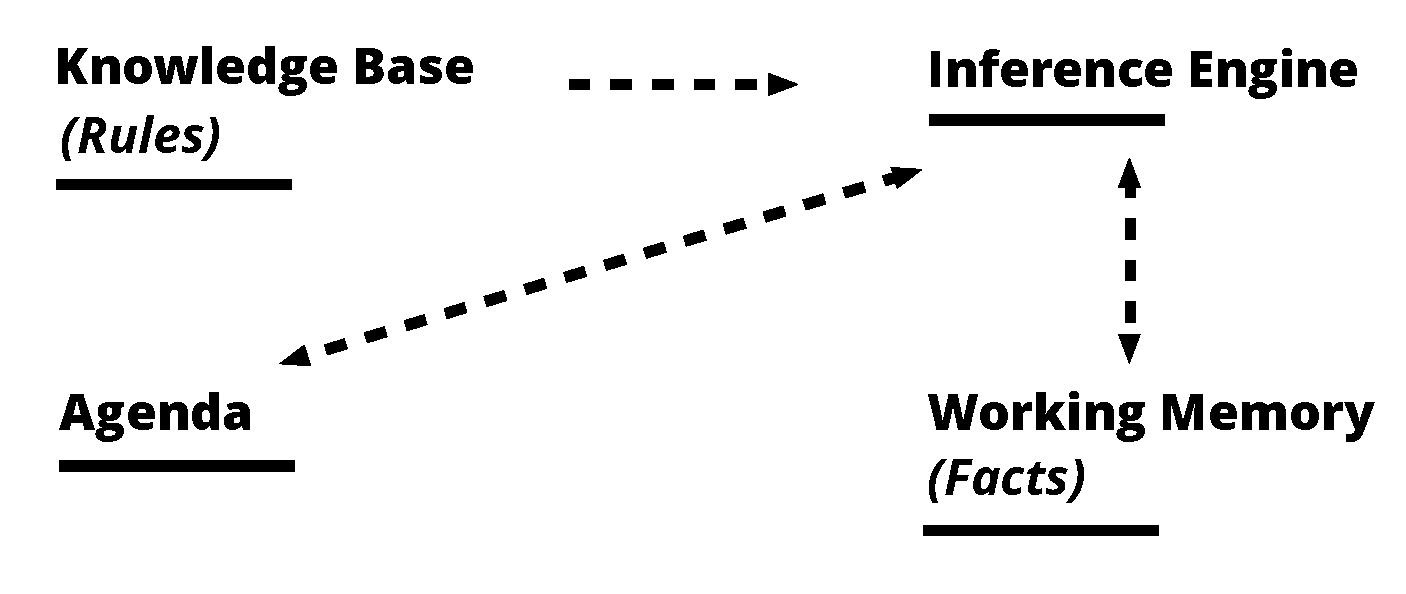
\includegraphics[width=0.8\textwidth]{Figures/es-arch}
  \end{center}
  
\end{frame}



{
  \begin{frame}[t]
    \frametitle{Expert System Shells}
    \framesubtitle{A little bit of history}
    \begin{table}
      \setlength\tabcolsep{2pt}
      \centering
      \begin{tabular}{c c c c}
        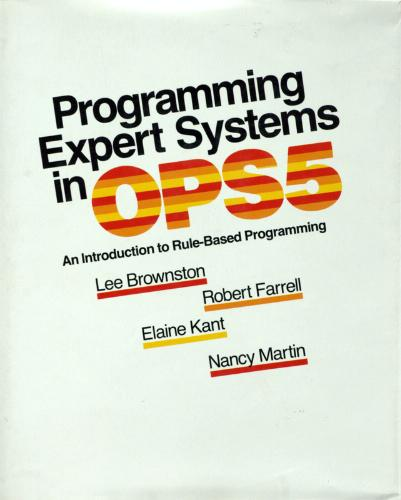
\includegraphics[width=70pt]{Figures/ops5} &
        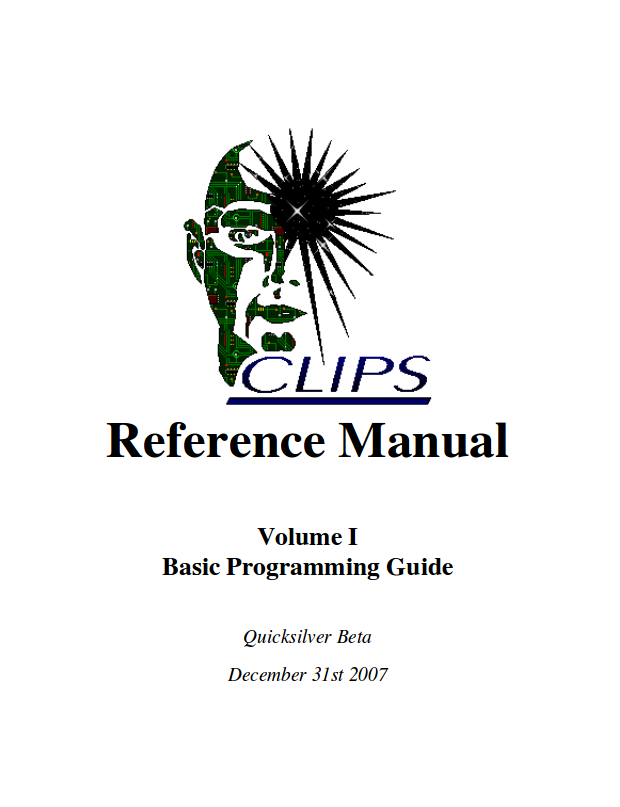
\includegraphics[width=70pt]{Figures/clips-programming} &
        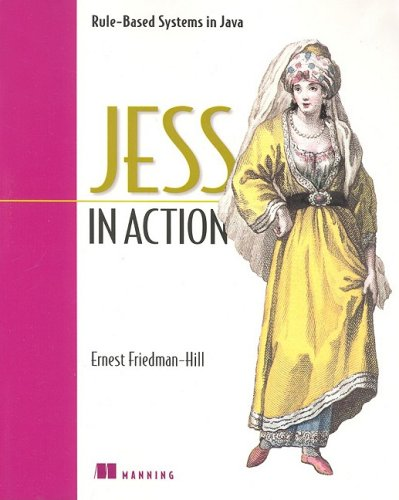
\includegraphics[width=70pt]{Figures/jess}&
        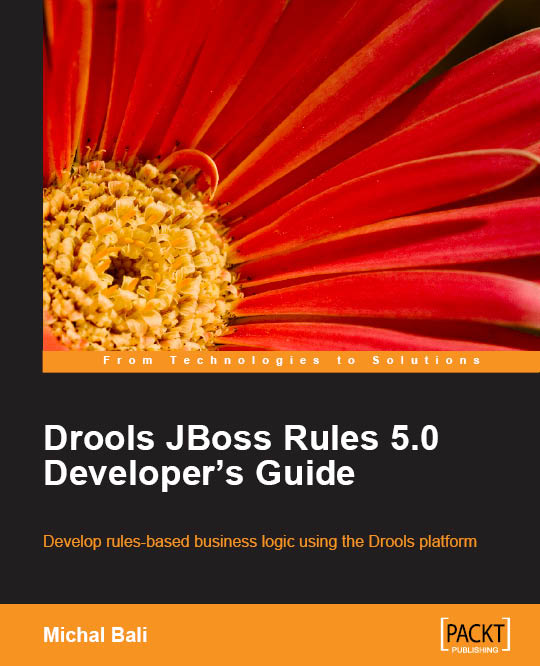
\includegraphics[width=70pt]{Figures/drools}\\
        \emph{1981} & \emph{1985} & \emph{1995}& \emph{2001}
      \end{tabular}
    \end{table}
    
  \end{frame}
}


\begin{frame}
  \frametitle{CLIPS}
  \textsf{C} \textsf{L}anguage \textsf{I}ntegrated \textsf{P}roduction
  \textsf{S}ystem.\par\bigskip
  A \textbf{forward chaining} rule language based on the \textbf{Rete} algorithm,
  created in 1985 at NASA's Johnson Space Center.\par\bigskip
  
  It became an \textbf{expert
  system shell}, i.e. an environment to write expert systems (it can also
be used for fast prototyping).\par\bigskip

  Written in \textsf{C}, but resembling \textsf{LISP} (\emph{embrace parentheses}!).\par\bigskip
  
  Multi-paradigmatic: \underline{rule programming} + \underline{functional programming}
  aspects + oop. Embeddable: C APIs (but also wrappers in Java,
  python, .Net\dots).\par\bigskip
  
  Current version \textsf{6.30}, released 2015/03/25, \textsf{6.24} is fine as well
  (installed in labs).
\end{frame}

\section{Applications}
{\setbeamertemplate{headline}{}
  \begin{frame}
    \sectionpage
  \end{frame}
}

\begin{frame}
  \frametitle{Formal Systems}
  \textbf{Formal languages} and \textbf{grammars} are an example of formal systems you
  already met. Rules encode how to produce or \emph{rewrite} symbolic
  knowledge.
  $$S\rightarrow ASb, A\rightarrow a, A\rightarrow \lambda$$\par\bigskip
  
  The first attempt to embed \emph{all mathematical truths} into a single
  formal system is to be found in \href{http://en.wikipedia.org/wiki/Principia_Mathematica}{Principia
    Mathematica} (1910-1927). We know \href{http://en.wikipedia.org/wiki/G\%C3\%B6del\%27s_incompleteness_theorems}{how it ended}\dots\par\bigskip
  
  Nowadays' applications are software theorem provers and model checking, exploited in formal software verification.
\end{frame}


\begin{frame}
  \frametitle{Expert Systems}
  \begin{table}[htbp]
    \centering
    %\setlength{\tabcolsep}{3pt}  
    \begin{tabular}{r l}
      %\toprule
      \textbf{Interpretation} & Hearsay (Speech Recognition), PROSPECTOR\\
      \textbf{Prediction} & Preterm Birth Risk Assessment \\
      \textbf{Diagnosis} & CADUCEUS, MYCIN, PUFF, Mistral, Eydenet, Kaleidos\\
      \textbf{Design} & Dendral, Mortgage Loan Advisor, R1\\
      \textbf{Planning} & Mission Planning for Autonomous Underwater Vehicle\\
      \textbf{Monitoring} & REACTOR\\
      \textbf{Debugging} & SAINT, MATHLAB, MACSYMA\\
      \textbf{Repair} & Toxic Spill Crisis Management\\
      \textbf{Intruction} & MH.PAL, Intelligent Clinical Training, STEAMER\\
      \textbf{Control} & Real Time Process Control, Space Shuttle Mission Control\\
      
      %\midrule
      
    \end{tabular}
    %\caption[datasets]{Datasets used and their statistics}
    %\label{tab:datasets}
  \end{table}\footnotenomarkleft{Hayes-Roth, F.; Waterman, D.; Lenat,
    D. Building Expert Systems. Addison-Wesley.1983}
  
  Not all are rule-based.
\end{frame}

\begin{frame}[fragile,fragile]
  \frametitle{Soar}
  \href{http://soar.eecs.umich.edu/}{Soar} is a cognitive architecture, created by Laird, \emph{Newell},
  and Rosenbloom.\par\bigskip
  
  It is the embodiment of an intelligent agent system.\par\bigskip
  It is both a view of what cognition is and an implementation of that
  view through a programming architecture for AI modeling different aspects of human
  behavior.\par\bigskip
  It is based on a production system, it uses explicit \textbf{production
    rules} to govern its behavior. An example rule to model plan intentions\footnote{\url{http://people.ict.usc.edu/~traum/Talks/ict-dm-tutorial5.pdf}}:
  {\tiny
\begin{verbatim}

sp {top-ps*elaborate*task*belief*intend*true
   (state <s> ^problem-space.name top-ps ^agent-name <me> ^plan <task>)
   (<task> ^intend true ^responsibility <me> ^authorized yes)
-->
   (<task> ^belief true)
}
\end{verbatim}}
\end{frame}


\begin{frame}
  \frametitle{Rule based Game AIs}
  \begin{center}
    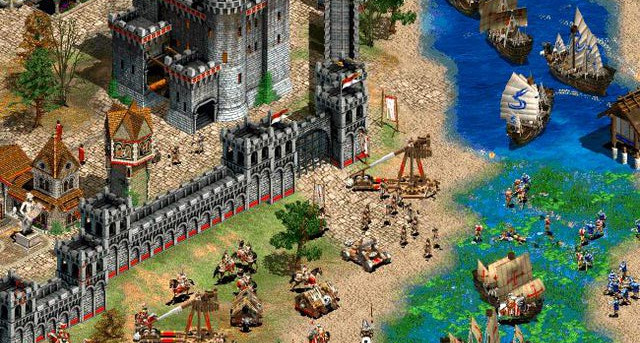
\includegraphics[width=1.0\textwidth]{Figures/aokii-crop}
  \end{center}
  \footnotenomarkleft{[2000] \href{http://cobweb.cs.uga.edu/~potter/aok/}{Microsoft - Age of Empires II: Age of Kings}}
\end{frame}

\section{Resources}
{\setbeamertemplate{headline}{}
  \begin{frame}
    \sectionpage
  \end{frame}
}

\begin{frame}
  \frametitle{Books}
  Please do not study from these slides.\par\bigskip
  
  
  \textbf{Expert Systems: Principles and Programming}\\
  \emph{J. Giarratano \& G. Riley}. Course Technology. \emph{4th
  Edition}. 2004.\\
  From the programmers of CLIPS, useful and general enough to get
  confidence with the language.
  \begin{flushright}
    \vspace{-5pt}
    \emph{Chapters 6-10, 12}
  \end{flushright}
  
  
  
  \textbf{Introduction to Expert Systems}\\
  \emph{Peter Jackson}. Addison-Wesley. \emph{Third Edition}. 1998.\\
  Less CLIPS-centric, but heavier on expert system design and
  implementation issues. It will come handy for the exam.
  \begin{flushright}
    \vspace{-5pt}
    Chapters 10-12, 16-17
  \end{flushright}
  
  
\end{frame}

\begin{frame}
  
  \frametitle{CLIPS Programming I}
  
  Assuming version \textsf{6.30}, there are equivalent for versione \textsf{6.24}.\par\bigskip
  
  
  \textbf{CLIPS User's Guide}\\
  Most of the basic arguments we will face can be found in this
  tutorial. A must.
  \begin{flushright}
    \vspace{-5pt}
    \href{http://clipsrules.sourceforge.net/documentation/v630/ug.pdf}{documentation/v630/ug.pdf}
  \end{flushright}
  
  
  
  \textbf{CLIPS Basic Programming Guide}\\
  It contains the documentation and examples for each shell and
  language construct.
  \begin{flushright}
    \vspace{-5pt}
    \href{http://clipsrules.sourceforge.net/documentation/v630/bpg.pdf}{documentation/v630/bpg.pdf}
  \end{flushright}
  
  
  \textbf{CLIPS Advanced Programming Guide}\\
  Explaining in depth the source code, the modules functioning and how to use CLIPS APIs from a wrapper program (in C).
   \begin{flushright}
    \vspace{-5pt}
    \href{http://clipsrules.sourceforge.net/documentation/v630/apg.pdf}{documentation/v630/apg.pdf}
  \end{flushright}
  
\end{frame}

\begin{frame}
  \frametitle{CLIPS Programming II}
  \scriptsize
  Projects for embedding CLIPS into external
  frameworks. Beware outdated software.\par\bigskip
  
  \textbf{clipsmm}\\
  C++ wrapper of CLIPS C APIs.
  \begin{flushright}
    \vspace{-20pt}
    \href{http://clipsmm.sourceforge.net/}{clipsmm@sourceforge}
  \end{flushright}
  \textbf{CLIPSnet}\\
  Embedding CLIPS in to .NET applications (bleargh).
  \begin{flushright}
    \vspace{-20pt}
    \href{http://sourceforge.net/projects/clipsnet/}{clipsnet@sourceforge}
  \end{flushright}
  \textbf{CLIPS .NET interface 0.1}\\
  Official .NET Interface for CLIPS. Better to leave it where it is\dots
  \begin{flushright}
    \vspace{-20pt}
    \href{http://www.clipsrules.net/?q=Downloads/CLIPSNET}{CLIPS-.NET@sourceforge}
  \end{flushright}
  \textbf{DROID-CLIPS}\\
  Porting CLIPS to Android.
  \begin{flushright}
    \vspace{-20pt}
    \href{https://github.com/DrItanium/DROID-CLIPS}{droid-clips@github}
  \end{flushright}
  \textbf{pyCLIPS}\\
  Python 2.X wrapper.
  \begin{flushright}
    \vspace{-20pt}
    \href{http://pyclips.sourceforge.net/web/}{pyclips@sourceforge}
  \end{flushright}
  \textbf{CLIPS JNI 0.5 \emph{beta}}\\
  Official Java Native Interface for CLIPS. We'll use it later in the course.
  \begin{flushright}
    \vspace{-20pt}
    \href{http://clipsrules.sourceforge.net/CLIPSJNIBeta.html}{CLIPS-JNI@sourceforge}
  \end{flushright}
  \textbf{CLIPSiOS 0.1}\\
  Official iOS Native Interface for CLIPS.
  \begin{flushright}
    \vspace{-20pt}
    \href{http://www.clipsrules.net/?q=Downloads/CLIPSiOS}{CLIPSiOS@sourceforge}
  \end{flushright}
  
\end{frame}

\begin{frame}
  \frametitle{Additional Resources}

  \textbf{CLIPS Forum}\\
  Sourceforge project discussion boards
  \begin{flushright}
    \vspace{-5pt}
    \href{http://sourceforge.net/p/clipsrules/discussion/}{CLIPS@sourceforge}
  \end{flushright}

  
  \textbf{CLIPSESG}\\
  CLIPS Expert System Group, a much more updated forum for users to
  ask for help and interact.
  \begin{flushright}
    \vspace{-5pt}
    \href{https://groups.google.com/forum/\#!forum/CLIPSESG}{CLIPSESG@googlegroups}
  \end{flushright}
  
\end{frame}

\section{Exam}
{\setbeamertemplate{headline}{}
  \begin{frame}
    \sectionpage
  \end{frame}
}



\end{document}

%%% Local Variables:
%%% mode: latex
%%% TeX-engine: xetex
%%% TeX-master: t
%%% End:
